\documentclass[xcolor=dvipsnames]{beamer}

% 1. PREÁMBULO: Configuraciones Globales
\usetheme{Madrid}
\usepackage[utf8]{inputenc}
\usepackage[spanish, es-tabla]{babel} % es-tabla para que diga Tabla y no Cuadro
\usepackage{amsmath, amssymb}
\usepackage{diagbox}
\usepackage{multirow}
\usepackage{tikz}

% 2. CONFIGURACIÓN DE TIKZ (Debe ir en el preámbulo)
\usetikzlibrary{arrows.meta, positioning, calc}
\tikzset{
    state/.style={circle, draw=black, thick, minimum size=1.1cm, font=\bfseries},
    alc/.style={state, fill=Emerald!20, text=Emerald!70!black},
    baj/.style={state, fill=Maroon!20, text=Maroon!70!black},
    est/.style={state, fill=Gray!20, text=Gray!70!black},
    trans/.style={->, >={Stealth[scale=1.0]}, thick, black!70, shorten >=1pt},
    val/.style={font=\tiny\bfseries, text=blue!80!black, yshift=2mm}
}

\title{Toma de Decisiones Secuenciales \\ y Aprendizaje por Refuerzo}
\author{Daniela Pucci de Farias}
\institute{Universidad Torcuato Di Tella}
\date{Modulo 1: Intro y MRPs}

% 3. PERSONALIZACIÓN DEL FOOTER (Muestra únicamente: Módulo | Páginas con margen izquierdo)
\setbeamertemplate{footline}{
  \leavevmode%
  \hbox{%
  % Bloque 1 (Izquierda/Centro): Nombre del Módulo con más espacio al borde (leftskip)
  \begin{beamercolorbox}[wd=.8\paperwidth,ht=2.25ex,dp=1ex,leftskip=4ex,left]{title in head/foot}%
    \usebeamerfont{title in head/foot}\hspace*{2ex} \insertdate
  \end{beamercolorbox}%
  % Bloque 2 (Derecha): Numeración de Páginas
  \begin{beamercolorbox}[wd=.2\paperwidth,ht=2.25ex,dp=1ex,right]{date in head/foot}%
    \usebeamerfont{date in head/foot}
    \insertframenumber{} / \inserttotalframenumber\hspace*{2ex} 
  \end{beamercolorbox}}%
  \vbox{}%
}

\begin{document}

% --- SLIDE 1: PORTADA ---
\frame{\titlepage}

\begin{frame}{Contenidos del Curso}
\begin{itemize}
\item \textbf{Modelado y resolución de problemas de toma de decisiones secuenciales bajo incertidumbre.}
\item<2->  \textbf{Programa}
\begin{itemize}
\item<2->  \textbf{M\'odulo 1: Procesos markovianos y procesos markovianos con recompensa.}
\begin{itemize}
\item Aplicaciones a control de stock, regímenes de mercado y análisis de participación de empresas en el mercado.
\end{itemize}

\item<3-> \textbf{M\'odulo 2: Procesos markovianos de decisión (MDPs).}  
\begin{itemize}
\item Aplicaciones a precificación dinámica, gesti\'on de recursos y optimización de portafolios. 
\end{itemize}

\item<4->  \textbf{M\'odulo 3: Aprendizaje por refuerzo.} 
\begin{itemize}
\item Aplicación a problemas de navegación y precificación de opciones.
\end{itemize}
\end{itemize}
\end{itemize}   
\end{frame}

\begin{frame}{Criterio de Evaluación}
La nota estará basada en el siguiente esquema de ponderación: 
\begin{itemize}
\item Participación en clase, asistencia y puntualidad: 10\%
\item<2-> Trabajo práctico grupal: 40\% 
\begin{itemize}
\item<3-> formación de los grupos: 8 de junio 
\item<3-> Propuesta de proyecto: 29 de junio
\item<3-> Presentación oral (15 minutos) y relatorio final: 27 de julio
\end{itemize}
\item<4-> Tareas individuales (4 tareas): 50\%
\begin{itemize}
\item<5-> Tarea 1: asignada el 2 de junio, fecha de entrega el 9 de junio
\item<5-> Tarea 2: asignada el 9 de junio, fecha de entrega el 16 de junio
\item<5-> Tarea31: asignada el 23 de junio, fecha de entrega el 30 de junio
\item<5-> Tarea 2: asignada el 30 de junio, fecha de entrega el 7 de julio
\end{itemize}
\item<6-> Tareas y código python (Google Colab) deben ser entregados por el campus virtual
\end{itemize}
\end{frame}

% --- SLIDE 4: DEFINICIÓN ---
\begin{frame}{¿Qué es una Decisión Secuencial?}
\begin{center}
    \Large ``¿Qué creen que significa?''
\end{center}
\pause


    \begin{itemize}
        \item \textbf{Ejemplo:``¿compro esta casa o no?' } 
        \begin{itemize}
            \small
            \item<3-> No es una decisión aislada.
            \item<4-> El problema secuencial \textbf{considera una decisi\'on y su impacto en el futuro}: ``¿compro hoy o sigo buscando?'' o ``¿compro o ahorro para el futuro?''.
	  \item<5-> Incertidumbres son incorporadas.
	  \item<6-> Cada acci\'on puede utilizar informaci\'on disponible hasta el momento en que debe ser tomada.
        \end{itemize}
        
        \item<7-> \textbf{Dependencia Temporal y Dinámica:} 
        \begin{itemize}
            \small
            \item La acción de hoy depende de lo que ha pasado anteriormente y altera las opciones disponibles mañana.
            \item El entorno evoluciona con incertidumbre.
        \end{itemize}
    \end{itemize}

\end{frame}

% --- SLIDE 5: CASO DINÁMICO VS ESTÁTICO ---
\begin{frame}{Ejemplo: Gesti\'on de Stock}
\begin{columns}
\begin{column}{0.5\textwidth}
\textbf{Visión Mi\'opica:}
"{}Optimiza el pedido de hoy para minimizar el costo de hoy."

o 

\textbf{Visión Est\'atica:}
"{}Planifica una secuencia rígida de acciones futuras basándose únicamente en la información disponible hoy."
\end{column}
\begin{column}{0.5\textwidth}
\textbf{Visión Secuencial:}
"{}Si pido de más hoy, tendré costos de almacenamiento mañana; si pido de menos, perderé clientes bajo incertidumbre. Decido hoy considerando ese impacto futuro, sabiendo que mañana podré ajustar mi decisión con la nueva información disponible."
\end{column}
\end{columns}
\vspace{0.5cm}
\begin{block}{Insight}
Las decisiones secuenciales consideran el \textbf{Costo de Oportunidad} del futuro y se adaptan din\'amicamente   la informaci\'on que va siendo revelada.
\end{block}
\end{frame}

\begin{frame}{Resumiendo: en toma de decisiones secuenciales...}
\begin{itemize}
\item Las decisiones se toman a lo largo del tiempo.
\item Están sujetas a incertidumbre.
\item Tienen impacto sobre posibilidades y resultados futuros.
\end{itemize}
\end{frame}

% --- SLIDE 3: EJEMPLOS (Original style) ---
\begin{frame}{¿Dónde se utiliza?}
\begin{itemize}
\item<1-> Ejemplos:
\begin{itemize}
\item precios dinámicos
\item decisiones de inversión
\item gestión de stock
\item control de producción
\item agentes que interactúan con un entorno
\end{itemize}
\item<2->Una pregunta:
\begin{center}
¿Cómo estructuramos estos problemas?
\end{center}
\item<3-> Idealmente:
\begin{center}
\Large
\textbf{un único marco que sirva para todos}
\end{center}
\end{itemize}
\end{frame}

\begin{frame}
\frametitle{El Marco: Agente y Ambiente}
 \centering
 \mode<beamer>{
    \only<1>{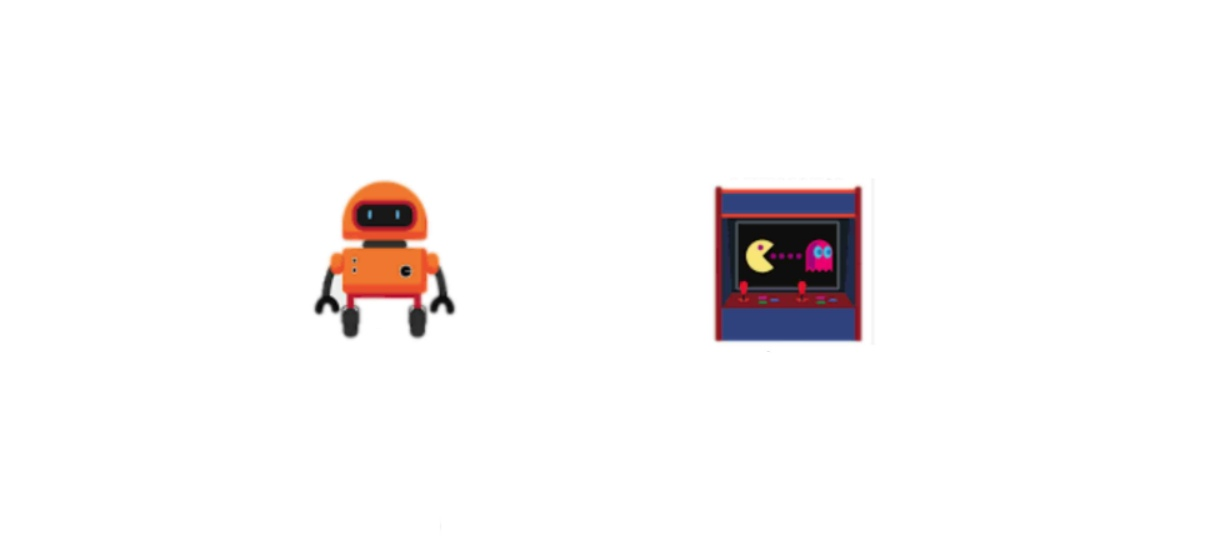
\includegraphics[width=1\textwidth]{../Images/RL/RL0.jpg}}
    \only<2>{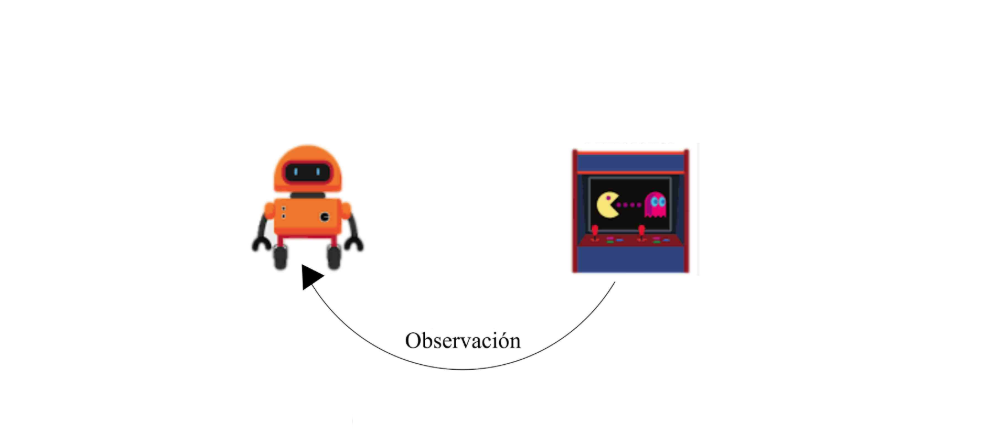
\includegraphics[width=1\textwidth]{../Images/RL/RL1.png}}
    \only<3>{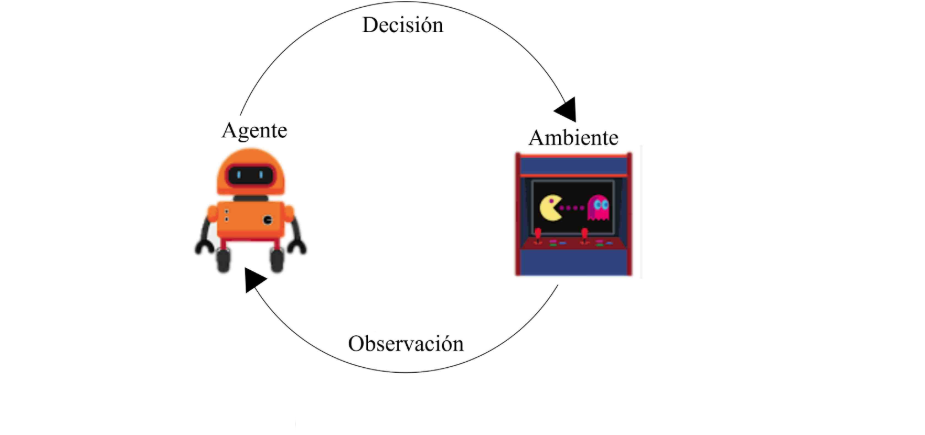
\includegraphics[width=1\textwidth]{../Images/RL/RL2.png}}}
    \only<4->{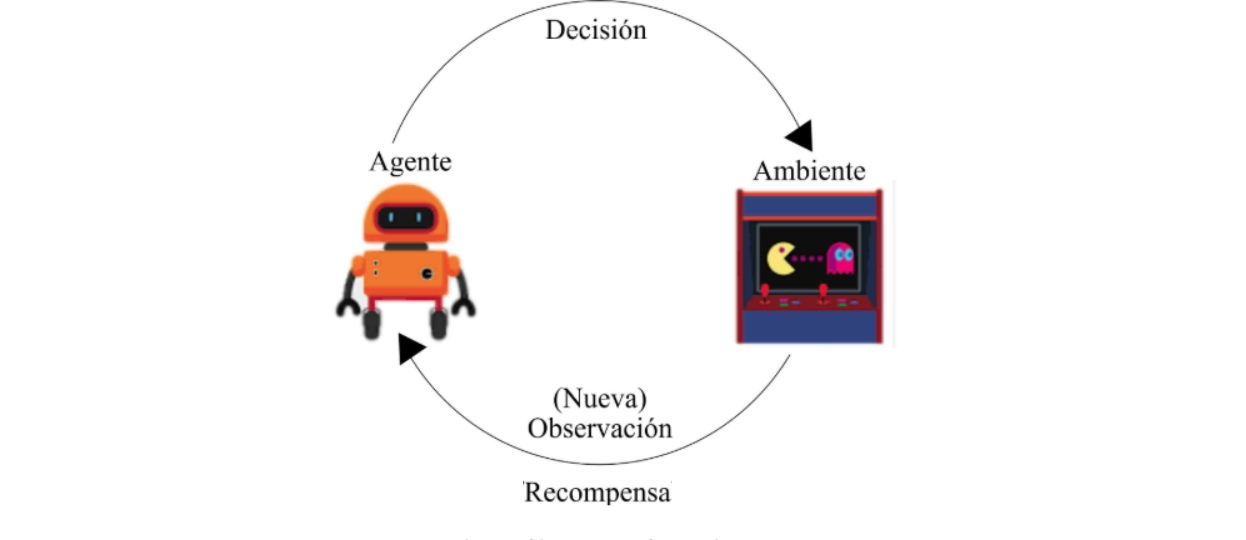
\includegraphics[width=1\textwidth]{../Images/RL/RL3_new.jpg}}
\only<5>{\textquestiondown C\'omo representar el problema matem\'aticamente?}
\end{frame}

% --- NUEVA SLIDE: INTRODUCCIÓN A MDP ---
%\begin{frame}{Procesos de Decisión de Markov (MDP)}
%Para representar estos problemas matemáticamente, utilizamos los \textbf{MDPs}.
%\begin{itemize}
%    \item Es el formalismo estándar para la toma de decisiones secuenciales.
%    \item \textbf{El objetivo:} Encontrar una \textit{política} (regla de decisión) que maximice la recompensa acumulada en el tiempo.
%\end{itemize}
%\begin{block}{Componentes del MDP}
%\begin{enumerate}
%    \item \textbf{Estados ($S$):} Todas las situaciones posibles.
%    \item \textbf{Acciones ($A$):} Todas las decisiones posibles.
%    \item \textbf{Transiciones ($P$):} La dinámica del ambiente (probabilidades).
%    \item \textbf{Recompensas ($R$):} El feedback del ambiente.
%\end{enumerate}
%\end{block}
%\end{frame}
%
%% --- SLIDE 5: EJEMPLO CONCRETO (Mapping MDP) ---
%\begin{frame}{Ejemplo: Control de Stock como MDP}
%Mapeo de los componentes al problema de inventario:
%
%\begin{itemize}
%    \item \textbf{Estado ($s_t$):} 
%        \alt<handout>{\hspace{4cm} }{ \only<2->{\textcolor{blue}{Stock actual en depósito.}} }
%        
%    \item \textbf{Acción ($a_t$):} 
%        \alt<handout>{ \hspace{4cm} }{ \only<2->{\textcolor{blue}{Cantidad a pedir al proveedor.}} }
%        
%    \item \textbf{Transición ($P$):}  
%        \alt<handout>{\hspace{3cm} }{ \only<2->{Determinada por la \textcolor{blue}{\textbf{Demanda aleatoria}.}} }
%    \alt<handout>{\hspace{3cm}}{
%    \begin{itemize}
%        \item<2-> \textit{\textcolor{blue}{Ej: Si $s_t=10$ y pido $a_t=5$, pero el mercado demanda $8 \to s_{t+1}=7$.}}
%    \end{itemize}}
%
%    \item \textbf{Recompensa ($r_t$):} 
%        \alt<handout>{ \hspace{5cm} }{ \only<2->{\textcolor{blue}{Margen neto (ventas - costos).}} }
%\end{itemize}
%
%\begin{center}
%\begin{tikzpicture}[node distance=1.6cm, auto, thick, scale=0.8, every node/.style={scale=0.8}]
%    \node [rectangle, draw, minimum width=2.5cm, fill=blue!10] (agent) {Manager};
%    \node [rectangle, draw, minimum width=2.5cm, below of=agent, fill=gray!10] (env) {Ambiente (Mercado)};
%    
%    \draw [-Stealth] (agent.east) -- ++(1,0) |- node [near start, right] {Acción $a_t$} (env.east);
%    \draw [-Stealth] (env.west) -- ++(-1,0) |- node [near start, left] {$\begin{array}{c} s_t \\ s_{t+1}, r_t \end{array}$} (agent.west);
%\end{tikzpicture}
%\end{center}
%
%\begin{block}{El Objetivo}
%    \alt<handout>{
%        ¿Qué buscamos optimizar? 
%    }{
%        \only<1>{¿Qué buscamos optimizar?}
%        \only<2->{\textcolor{blue}{Maximizar la ganancia acumulada decidiendo cuánto pedir hoy.}}
%    }
%\end{block}
%\end{frame}
%
%
%
%% --- NUEVA SLIDE: DESAFÍOS DE IMPLEMENTACIÓN ---
%\begin{frame}{Desafíos al aplicar la metodología}
%\begin{itemize}
%    \item \textbf{Modelado conceptual:}
%    \begin{itemize}
%        \item \textbf{Diseño del Estado:} Identificar qué información es suficiente para la toma de decisiones.
%        \item \textbf{Diseño de la Recompensa:} Alinear incentivos para evitar comportamientos indeseables del agente.
%    \end{itemize}
%    
%    \item \textbf{Incertidumbre (Parámetros desconocidos):}
%    \begin{itemize}
%        \item Si no conocemos la dinámica del mercado, pasamos al \textbf{Aprendizaje por Refuerzo}.
%    \end{itemize}
%
%    \item \textbf{Desafíos Computacionales:}
%    \begin{itemize}
%       \item  \textquestiondown C\'omo encontrar decisiones que maximicen la recompensa?
%        \item \textbf{Maldición de la Dimensionalidad:} El número de estados crece exponencialmente con las variables (ej: múltiples productos). Algoritmos de aproximación se vuelven necesarios.
%    \end{itemize}
%\end{itemize}
%\end{frame}

% --- SLIDE: HOJA DE RUTA ---
\begin{frame}{El Marco Matem\'atico: Jerarquía de Modelos}
Para representar estos problemas matemáticamente, utilizamos los \textbf{procesos markovianos de decisi\'on (MDPs)}.
\begin{itemize}
    \item Es el formalismo estándar para la toma de decisiones secuenciales.
\item Para dominar los MDPs, iremos de lo más simple (sistemas pasivos) a lo más complejo (sistemas con control):
\begin{enumerate}
    \item \textbf{Procesos markovianos:} Solo dinámica. El sistema evoluciona solo.
    \item \textbf{Procesos markovianos con recompensa (MRP):} Dinámica + Recompensas (evaluación).
    \item \textbf{Procesos markovianos de decisi\'on (MDP):} Dinámica + Recompensas + \textbf{Control}.
\end{enumerate}
\end{itemize}
\vspace{0.3cm}
\begin{block}{Hoy: Procesos markovianos}
Modelaremos la evolución de sistemas aut\'onomos integrando la incertidumbre, utilizando los \textbf{procesos markovianos} para formalizar el cambio y el azar.
\end{block}
\end{frame}

% --- SLIDE: MODELANDO UN AMBIENTE AUTÓNOMO ---
\begin{frame}{Modelando un Ambiente Autónomo}
\begin{itemize}
    \item \textbf{Ejemplo:} ¿Cómo representar condiciones de mercado?
    \item<2-> En cada semana, el mercado se encuentra en uno de tres estados posibles.
    \item<3-> ¿Cómo evolucionan en el tiempo? 
    \begin{itemize}
        \item<4-> Descripción probabilística utilizando grafos (\textbf{nodos} = estados, \textbf{arcos} = transiciones).
        \item<5-> Nos enfocaremos en procesos a tiempo discreto: \textbf{procesos markovianos}.
    \end{itemize}
\end{itemize}

\centering
\mode<beamer>{
    \only<2>{
\includegraphics[width=0.75\textwidth]{../Images/Market/Market1.png}}
    \only<3>{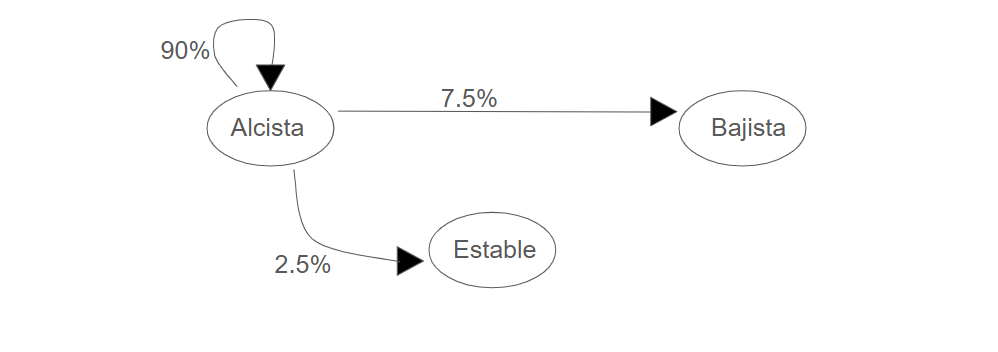
\includegraphics[width=0.75\textwidth]{../Images/Market/Market2.png}}
    \only<4>{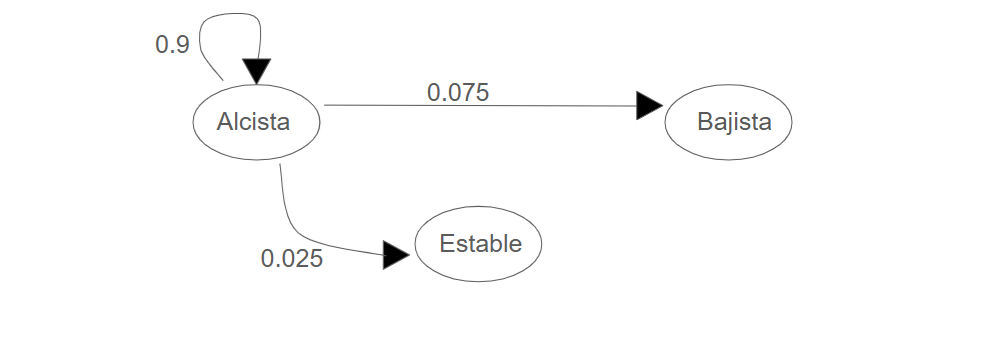
\includegraphics[width=0.75\textwidth]{../Images/Market/Market3.png}}
    \visible<5->{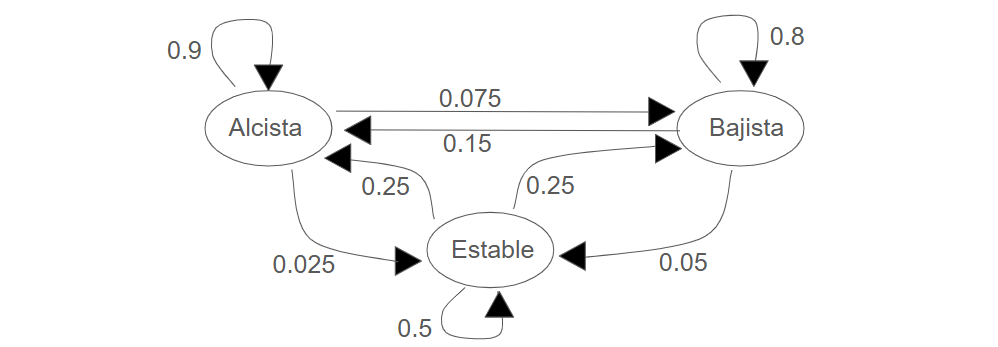
\includegraphics[width=0.75\textwidth]{../Images/Market/Market4.png}}
}
\end{frame}

% --- SLIDE: PROCESOS MARKOVIANOS (DEFINICIÓN) ---
\begin{frame}{Procesos Markovianos}
¿Cómo definir matemáticamente el proceso de regímenes de mercado?

\begin{columns}[t]
    \begin{column}{0.62\textwidth}
        \begin{itemize}
            \item<2-> \textbf{Espacio de estados $S$}
            \begin{itemize}
                \item $S = \{\text{Alcista, Bajista, Estable}\}$
                \item Los estados pueden ser discretos o continuos.
            \end{itemize}
            
            \item<3-> \textbf{Matriz de transición $P$}
            \mode<beamer>{
                \only<3-7>{
                    \vspace{0.5em}
                    \small
                    \begin{tabular}{|l|c|c|c|}
                    \hline
                    \textbf{de / a} & \textbf{Alcista} & \textbf{Bajista} & \textbf{Estable} \\ \hline
                    Alcista & \visible<4-7>{0.9} & \visible<5-7>{0.075} & \visible<6-7>{0.025} \\ \hline
                    Bajista & \visible<7>{0.15} & \visible<7>{0.8} & \visible<7>{0.05} \\ \hline
                    Estable & \visible<7>{0.25} & \visible<7>{0.25} & \visible<7>{0.5} \\ \hline
                    \end{tabular}
                }
            }
            
            \only<8->{ 
            \[ P = \begin{bmatrix} 
            0.9 & 0.075 & 0.025 \\ 
            0.15 & 0.8 & 0.05 \\ 
            0.25 & 0.25 & 0.5 
            \end{bmatrix} \]}
        \end{itemize}
    \end{column}

    \begin{column}{0.35\textwidth}
        \centering
        \mode<beamer>{
            \only<1,3>{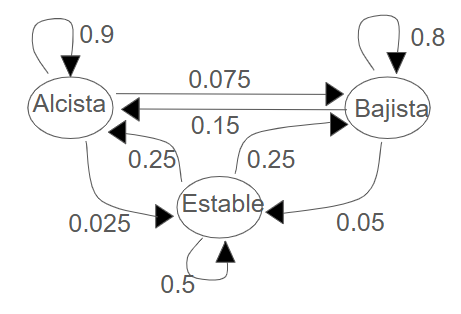
\includegraphics[width=\textwidth]{../Images/MarkovProcess/MarkovProcess1.png}}
            \only<2>{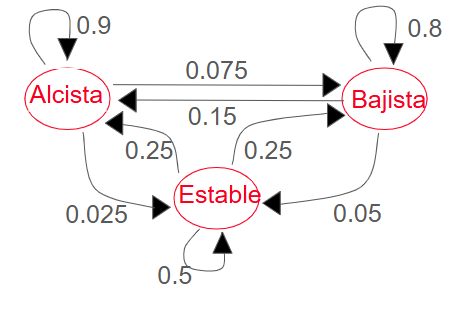
\includegraphics[width=\textwidth]{../Images/MarkovProcess/MarkovProcess2.png}}
            \only<4>{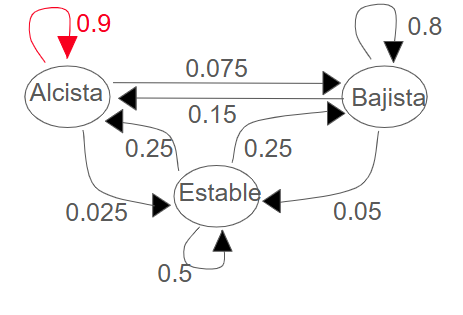
\includegraphics[width=\textwidth]{../Images/MarkovProcess/MarkovProcess3.png}}
            \only<5>{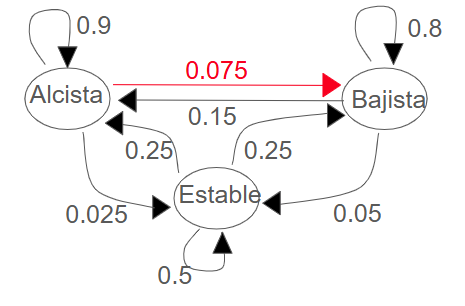
\includegraphics[width=\textwidth]{../Images/MarkovProcess/MarkovProcess4.png}}
            \only<6>{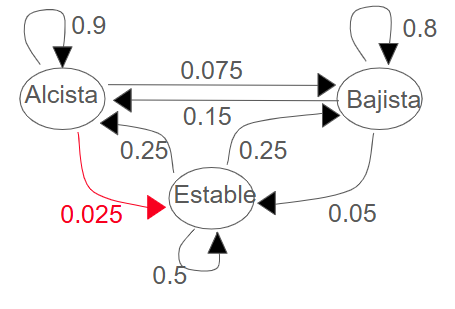
\includegraphics[width=\textwidth]{../Images/MarkovProcess/MarkovProcess5.png}}
            \only<7->{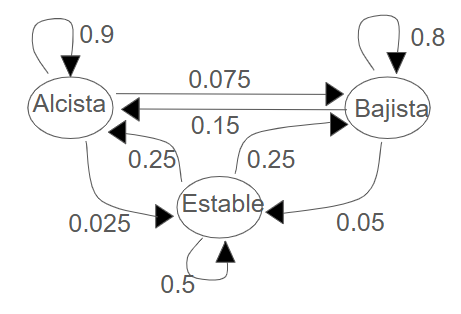
\includegraphics[width=\textwidth]{../Images/MarkovProcess/MarkovProcess1.png}}
        }
    \end{column}
\end{columns}

\vspace{0.5em}
\visible<9->{
    \begin{block}{Definición Fundamental}
        La tupla \textbf{$(S, P)$} define el proceso markoviano.
        Si $S$ es finito, lo denominamos \textbf{cadena de Markov}.
    \end{block}
}
\end{frame}

% --- SLIDE: MOTIVACIÓN (PREGUNTAS CLAVE) ---
\begin{frame}{Predicción en el Tiempo}
Supongamos que hoy observamos que el mercado es \textbf{Bajista}. Como responsables de una estrategia de inversión o logística, necesitamos proyectar el estado del sistema en distintos horizontes:

\begin{itemize}
    \item \textbf{Corto Plazo (Persistencia e Inercia):} 
    ¿Qué tan probable es que el mercado \textit{siga} siendo bajista la próxima semana? ¿Cambia mucho esa probabilidad en la semana 2?
    
    \item<2-> \textbf{Mediano Plazo (Disipación de la Información):} 
    A medida que miramos más lejos (ej. semanas 4 u 8), ¿la condición inicial de hoy sigue pesando, o el sistema se vuelve más impredecible?
    
    \item<3-> \textbf{Largo Plazo (Comportamiento Estructural):} 
    En el límite, cuando el tiempo tiende a infinito, ¿las probabilidades dependen de dónde empezamos hoy, o convergen a un equilibrio estable del mercado?
\end{itemize}


\end{frame}

% --- SLIDE: DISTRIBUCIÓN PROBABILÍSTICA (INTRODUCCIÓN) ---
\begin{frame}{Distribución Probabilística de Estados}
Representamos la probabilidad de estar en cada estado en el tiempo $t$ con el vector $\pi_t$: 
$$\pi_t(s) = \text{Prob}(s_t = s)$$

\visible<2->{En nuestro ejemplo, si hoy ($t=0$) el mercado es \textbf{Bajista}:}
\visible<3->{
$$ \pi_0 = \begin{bmatrix} 0 & 1 & 0 \end{bmatrix} $$
}
\visible<4-> {\textquestiondown C\'omo evolucionan esas probabilidades en el tiempo?}


\end{frame}

% --- SLIDE: CÁLCULOS PASO A PASO ---
\begin{frame}{Evolución de la Incertidumbre}
Si esta semana es \textbf{Bajista}, ¿cuál es la probabilidad de ser bajista en el futuro?
\begin{columns}[t]
\begin{column}{0.55\textwidth}
\vspace{-2.8cm} % Ajustá este valor según la altura de tu columna izquierda

\begin{itemize}
   \setlength{\itemsep}{0.1cm} % Controla de forma idéntica la separación entre preguntas
    
    \item \textbf{En la próxima semana ($t=1$)?}
    \uncover<2->{
        %\alt<handout>{\vspace{0.6cm}}{$$\pi_1 = [0.15 \,\, \mathbf{0.8} \,\, 0.05]$$}
$$\pi_1 = [0.15 \,\, \mathbf{0.8} \,\, 0.05]$$
    }
    
    \item \textbf{En 2 semanas ($t=2$)?}
    \uncover<4->{
        %\alt<handout>{\vspace{0.6cm}}{$$\pi_2 = [0.267 \,\, \mathbf{0.663} \,\, 0.068]$$}
$$\pi_2 = [0.267 \,\, \mathbf{0.663} \,\, 0.068]$$
    }
    
    \item \textbf{En 10 semanas ($t=10$)?}
    \uncover<7->{
       % \alt<handout>{\vspace{0.6cm}}{$$\pi_{10} = \pi_0 P^{10} \approx [0.591 \,\, \mathbf{0.343} \,\, 0.065]$$}
$$\pi_{10} = \pi_0 P^{10} \approx [0.591 \,\, \mathbf{0.343} \,\, 0.065]$$
    }
\end{itemize}

\end{column}
\begin{column}{0.45\textwidth}
\centering
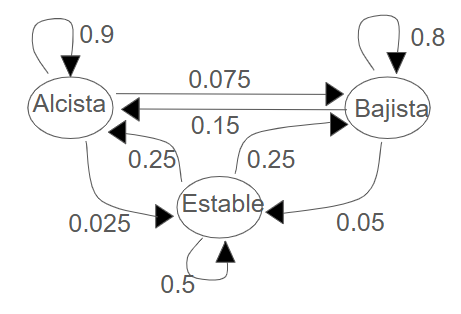
\includegraphics[width=0.9\textwidth]{../Images/MarkovProcess/MarkovProcess1.png}

\only<6->{%{\alt<handout>{}{
    \vspace{1.2cm} % Un pequeño respiro vertical antes del bloque
    % Forzamos un contenedor centrado del 90% del ancho de la columna
    \begin{minipage}{0.9\textwidth}
        \begin{alertblock}{Dinámica del Sistema}
        \centering
        $\pi_{t+1} = \pi_t P$ \\[0.1cm]
        Por inducción: $\pi_t = \pi_0 P^t$
        \end{alertblock}
    \end{minipage}
}%}
\end{column}
\end{columns}

\end{frame}

% --- SLIDE: DISTRIBUCIÓN ESTACIONARIA ---
\begin{frame}{Distribución Estacionaria}
¿Cuál es la frecuencia de largo plazo de cada régimen en este mercado?
\visible<2->{Buscamos la \textbf{distribución estacionaria} ($\pi$).}

\begin{itemize}
    \item<3-> Estacionariedad implica que el sistema ya no cambia: $\pi = \pi P$.
    \item<4-> Resolvemos el sistema sujeto a que las probabilidades sumen 1.
\end{itemize}

\visible<5->{
$$\pi_\infty = \lim_{t \to \infty} \pi_0 P^t \approx \begin{bmatrix} 0.625 & \mathbf{0.3125} & 0.0625 \end{bmatrix}$$
}

\visible<6->{
\begin{block}{Conclusión de Negocio}
A largo plazo, el mercado será \textbf{Alcista el 62.5\%} del tiempo, \textbf{Bajista el 31.25\%} y \textbf{Estable el 6.25\%}.
\end{block}
}
\end{frame}

% --- SLIDE: PROPIEDAD DE MARKOV (FORMALIZACIÓN) ---
\begin{frame}{Formalización: La Propiedad de Markov}
Para realizar los cálculos anteriores, hemos asumido algo crítico:
\begin{center}
\textit{"{}El futuro depende solo del estado presente, no de cómo llegamos a él."}
\end{center}

\begin{definition}[Propiedad de Markov]
$$P(s_{t+1} \mid s_t, s_{t-1}, \dots, s_0) = P(s_{t+1} \mid s_t)$$
\end{definition}

\vspace{0.3cm}
\textbf{Ejercicio de reflexión:}
¿Cambia la probabilidad de un mercado bajista la próxima semana si...
\begin{enumerate}
    \item ...llevamos 5 semanas en racha alcista?
    \item ...hoy es alcista, pero ayer fue un desastre bajista?
\end{enumerate}
\alt<handout>{ }{\visible<2->{\textcolor{blue}{Matemáticamente, si el estado actual es el mismo, la predicción es idéntica.}}}
\end{frame}


\begin{frame}{La Propiedad de Markov: Consecuencias}
Para realizar los cálculos anteriores, hemos asumido algo crítico:
\begin{center}
\textit{"{}El futuro depende solo del estado presente, no de cómo llegamos a él."}
\end{center}

\begin{definition}[Propiedad de Markov]
$$P(s_{t+1} \mid s_t, s_{t-1}, \dots, s_0) = P(s_{t+1} \mid s_t)$$
\end{definition}
\vspace{0.3cm}
\begin{itemize}
    \item Para un manager, esto simplifica la vida: no necesitamos recordar toda la historia de la empresa.
    \item \textbf{Solo importa el "hoy"}: Si el estado actual está bien diseñado, contiene toda la información necesaria para el futuro.
\end{itemize}
\end{frame}

% --- SLIDE: LA ELECCIÓN DEL ESTADO ---
\begin{frame}{La Elección del Estado: El Arte del Modelado}
El éxito de un modelo depende de qué incluimos (y qué omitimos) en el \textbf{Estado}.

\begin{itemize}
    \item<2-> \textbf{Suficiencia (Propiedad de Markov):}
    El estado debe ser un resumen de la historia que contenga \textit{toda} la información necesaria para predecir el futuro.
    \begin{itemize}
        \item \textcolor{red}{Riesgo:} Si falta información relevante, el modelo será incorrecto.
    \end{itemize}

    \item<3-> \textbf{Eficiencia (Maldición de la dimensionalidad):}
    Incluir información redundante aumenta el tamaño de $S$ innecesariamente.
    \begin{itemize}
        \item \textcolor{red}{Riesgo:} Complejidad computacional inmanejable.
    \end{itemize}

    \item<4-> \textbf{El Trade-off del Manager:}
    En la práctica, debemos balancear la precisión del modelo frente a la viabilidad de resolverlo.
\end{itemize}

\vspace{0.3cm}
\begin{exampleblock}{Reflexión: Regímenes de Mercado}<5->
En nuestro ejemplo, ¿es suficiente saber que hoy es Alcista? ¿Qué otras variables podr\'ian  influir en el cambio de estado?
\end{exampleblock}
\end{frame}

% --- SLIDE: DISCUSIÓN Y MODELADO COLABORATIVO ---
\begin{frame}{Debate: ¿Qué podemos modelar como procesos markovianos?}
\begin{block}{El Desafío}
Identifiquen procesos en distintas industrias (Energía, Logística, Finanzas, etc.) que sigan la lógica de "{}el presente basta para predecir el futuro".
\end{block}

\vspace{0.6cm}
\textbf{Enfoque del modelado:}
\begin{itemize}
    \item \textbf{Estado ($S$):} ¿Qué información mínima es indispensable hoy?
    \item \textbf{Transición ($P$):} ¿Qué eventos disparan el cambio?
    \item \textbf{Incertidumbre:} ¿De d\'onde surge?
\end{itemize}

\end{frame}

% ... [Continuar con el resto de las diapositivas: Ghana Telecom, Matrices, Recompensas, Lab, etc.] ...

% --- SLIDE: INTRODUCCIÓN A LA RECOMPENSA ---
\begin{frame}{Pero falta algo: La Valoración}
\begin{itemize}
    \item \textbf{Hasta ahora:} Sabemos cómo evoluciona el sistema (dinámica).
    \item<2-> \textbf{La realidad:} No todos los estados tienen el mismo valor para nosotros.
    \item<3-> \textbf{Necesidad:} Medir qué tan bueno es estar en un estado según nuestros objetivos.
\end{itemize}

\vspace{0.4cm}
\begin{center}
    \textit{Pasamos de describir el mundo a evaluarlo.}
\end{center}
\end{frame}

% --- SLIDE: FUNCIÓN DE RECOMPENSA ---
\begin{frame}{La Función de Recompensa}
En la toma de decisiones, buscamos alcanzar objetivos específicos:
\begin{itemize}
    \item<2-> Maximizar ganancias / Ingresos.
    \item<3-> Minimizar costos operativos / Riesgos.
    \item<4-> Cumplir metas (ej. ganar un juego o alcanzar un nivel de inventario).
\end{itemize}

\vspace{0.3cm}
\visible<5->{
    \begin{block}{Definición}
        Expresamos estos objetivos a través de la \textbf{función de recompensa $r(s)$}, que asigna un valor numérico inmediato a cada estado.
    \end{block}
}
\end{frame}

% --- SLIDE: MRP DEFINICIÓN ---
\begin{frame}{Proceso Markoviano con Recompensa (MRP)}
Formalmente, añadimos una nueva dimensión a nuestro modelo:
\begin{itemize}
    \item Proceso Markoviano: Tupla $(S, P)$
    \item<2-> \textbf{MRP:} Tupla $(S, P, r)$
    \begin{itemize}
        \item Donde \textbf{$r(s)$} es la recompensa (o costo) de estar en el estado $s$.
    \end{itemize}
\end{itemize}

\begin{center}
    \mode<beamer>{
        \only<3>{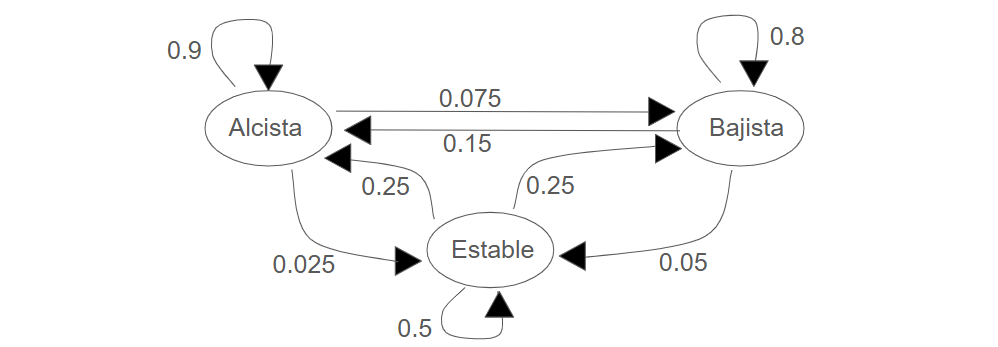
\includegraphics[width=0.7\textwidth]{../Images/Market/Market4.png}}
        \only<4->{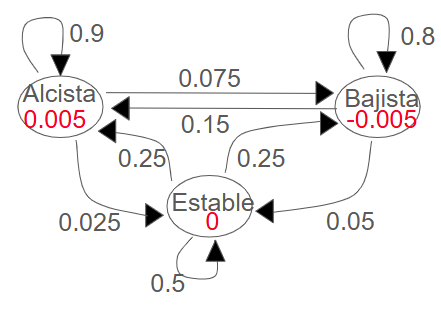
\includegraphics[width=0.45\textwidth]{../Images/Market/MarketWithReward.png}}
    }
\end{center}

\end{frame}



% --- SLIDE: EJEMPLO RECOMPENSA ---
\begin{frame}{Modelando el Valor del Mercado}
Definamos los retornos semanales para cada régimen de mercado:

\[
r(\text{Alcista}) = +0.005, \quad r(\text{Bajista}) = -0.005, \quad r(\text{Estable}) = 0
\]

\begin{itemize}
    \item<2-> $r(s) > 0$: Ganancia (incentivo).
    \item<2-> $r(s) < 0$: Costo o pérdida (penalidad).
\end{itemize}

\vspace{0.3cm}
\visible<3->{
    \begin{block}{Hacia la Evaluación}
        Con $r(s)$ definido, ya no solo predecimos el estado futuro, sino que podemos \textbf{evaluar trayectorias} completas de inversión.
    \end{block}
}
\end{frame}

% --- SLIDE: DISCUSIÓN - DESAFÍOS DE GESTIÓN DE INVENTARIO ---
\begin{frame}{Aplicaci\'on: Gestión de Stock}
Queremos evaluar nuestra estrat\'egia $n/N$ de gesti\'on de stock para compararla bajo distintos par\'ametros $n$y $N$.

¿Qué debemos considerar antes de formalizar el modelo?

\begin{enumerate}
    \item \textbf{Criterio de Optimalidad:} ¿Qu\'e costos y beneficios est\'an involucrados?
    \item \textbf{Estado:} ¿Basta saber el stock actual? ¿Qu\'e otros factores pueden ser importantes?
    \item \textbf{Incertidumbre:} ¿Modelo de demanda? ¿Otras fuentes de incertidumbre?
\end{enumerate}

\vspace{0.4cm}
\begin{block}{El Dilema del Modelador}
¿Qu\'e pasa al agregar m\'as y m\'as detalles al modelo? 

\textbf{Realismo vs Tratabilidad:} ¿Qué información sacrificarías primero para que el modelo sea resoluble?
\end{block}
\end{frame}

% --- SLIDE: COMPONENTES DEL MODELO (MRP) ---
\begin{frame}{Diseñando el MRP}
¿Cómo traducimos la realidad a un modelo MRP?

\begin{itemize}
    \item \textbf{Estado ($S$):} La "foto" del almacén. ¿Qué variables resumen la informaci\'on relevante del pasado?
    \item \textbf{Dinámica ($P$):} Transiciones de estado, impactadas por incertidumbre.
    \item \textbf{Recompensa ($R$):} ¿Costos y recompensas?
    \item \textbf{Horizonte ($T$):}  Planificación ¿mensual? ¿trimestral¿  ¿perpetua?
\end{itemize}

\end{frame}

% --- SLIDE: DISCUSIÓN - LA ARQUITECTURA DEL ESTADO ---
\begin{frame}{Discusión: ¿Qué constituye el estado?}
El estado $s$ debe contener \textbf{toda} la información necesaria para predecir el futuro.
\begin{itemize}
    \item \textbf{¿Qu\'e variables son importantes?} 
\end{itemize}

\vspace{0.3cm}


%\only<beamer| second | article>{
\begin{block}{Punto de Partida: Modelo Simplificado}<2->
     % Esto asegura que solo se vea en modos interactivos, no en handout puro si se configura así
    Para comenzar, asumiremos un entorno ideal:
    \begin{enumerate}
        \item \textbf{Demanda i.i.d.:} $D_t$ es independiente del pasado y sigue la misma distribución.
        \item \textbf{Entrega inmediata:} Cuando el nivel de stock baja a $n$,  se repone en el pr\'oximo periodo, volviendo a nivel $N$ ($Lead\ Time = 0$).
        \item \textbf{Estado:} $X_t \in \{0, 1, \dots, N\}$ (Solo el inventario actual).
    \end{enumerate}
\end{block}%}
\end{frame}
% --- SLIDE 2: MATRIZ DE TRANSICIÓN ---
\begin{frame}{Matriz de Transici\'on}
%\only<beamer>{
La transici\'on de estados est\'a dada por $X_{t+1} = f(X_t, D_t)$:
$$
X_{t+1} = \begin{cases} 
X_t - D_t & \text{if}~X_t-D_t > n \\
N & \text{if}~X_t-D_t \leq n
\end{cases}
$$
¿C\'omo convertimos la funci\'on $f(X_t, D_t)$ en una matriz de transici\'on $P$?

\visible<2->{
\begin{center}
\begin{tikzpicture}[node distance=1.2cm, auto, scale=0.7, every node/.style={transform shape}]
    \tikzset{
        state/.style={circle, draw=black, thick, minimum size=0.65cm, font=\small},
        dots/.style={minimum size=0.4cm},
        reorder/.style={circle, draw=blue, thick, fill=blue!5, minimum size=0.65cm, font=\small}
    }

    % Línea Superior: Decaimiento (j >= n)
    \node[state] (i) at (0,0) {$i$};
    \node[state] (i1) at (1.8,0) {$i-1$};
    \node[state] (i2) at (3.6,0) {$i-2$};
    \node[dots] (d) at (5.0,0) {$\dots$};
    \node[state] (n1) at (6.4,0) {$n+1$};

    % Línea Inferior: Reposición (Coordenada vertical reducida)
    \node[state] (N) at (3.8,-1.5) {$N$};

    % Transiciones de decaimiento
    \draw[->, >=stealth, loop above, black!60] (i) edge node {\tiny $D=0$} (i);
    \draw[->, >=stealth, black!60] (i) -- (i1) node[midway, above] {\tiny $D=1$};
    \draw[->, >=stealth, black!60] (i) to[bend left=35] node[midway, above] {\tiny $D=2$} (i2);
    \draw[->, >=stealth, black!60] (i) to[bend left=45] node[pos=0.8, above] {\tiny $D=i-n-1$} (n1);
    
    % Transición de reposición
    \draw[->, >=stealth,black!60] (i) -- (N) node[midway, left, font=\tiny] {$D \geq i-n$};
\end{tikzpicture}
\end{center}

\vspace{-0.2cm} % Ajuste sutil para recuperar espacio
\textbf{Mapeo de Probabilidades:}
%\mode<beamer>{
    \begin{itemize}
        \small
        \item<3-> \textbf{Si $n+1 \leq  j \leq i$:} $P_{ij} = \mathbb{P}(D_t = i-j)$ 
        \item<4-> \textbf{Si $j = N$:} $P_{iN} = \mathbb{P}(D_t \geq  i-n)$
    \end{itemize}
%}
%\mode<handout>{
  %  \vspace{1cm}
%}
}%}
\end{frame}

% --- SLIDE 3: FUNCIÓN DE RECOMPENSA ---
\begin{frame}{La Funci\'on de Recompensa}

%\only<beamer>{
La recompensa inmediata $r(X_t, D_t)$ balancea los ingresos operativos con los costos de estructura en cada periodo $t$:
{\small
$$
r(X_t, D_t) = \underbrace{p \cdot \min(X_t, D_t)}_{\text{Ventas}} - \underbrace{h \cdot X_t}_{\text{Stock}} - \underbrace{\pi \cdot \max(0, D_t - X_t)}_{\text{Quiebre}} - \underbrace{K \cdot \mathbb{I}(X_t - D_t \leq n)}_{\text{Orden}}
$$
}
\vspace{0.1cm}
Donde los parámetros económicos están definidos por:
\begin{itemize}
    \item $p$: Precio de venta unitario.
    \item $h$: Costo unitario de mantener inventario (bodega, seguros, capital inmovilizado).
    \item $\pi$: Penalidad por demanda insatisfecha ($\pi > p$).
\end{itemize}
\pause
La recompensa en ese caso no depende solo del estado sino tambi\'en de la demanda. Pero la podemos remplazar por
$$
r(s) = {\rm E}_D\left[ r(s,D) \right]
$$
%}
\end{frame}

% --- SLIDE: EVALUANDO MRPs ---
\begin{frame}{Evaluando MRPs}

Dada una situaci\'on formalizada como un Proceso de Recompensa de Markov (MRP), nos interesa cuantificar las ganancias o costos esperados en el tiempo:

\begin{itemize}
    \item \textbf{Retorno Esperado bajo Cambios de R\'egimen:} Si invertimos \$1 en el mercado bajo las condiciones actuales, ¿cu\'al es el retorno acumulado esperado al cabo de un horizonte de 3 semanas?
    \item \textbf{An\'alisis de Pol\'iticas Fijas:} Considerando un horizonte de planeaci\'on de 3 meses, qu\'e parametrizaci\'on de control de stock es mejor como una estrategia $(s, S)$,  ¿$(10,100)$ o $(25, 75)$?
\end{itemize}

\vspace{0.3cm}
A continuaci\'on, desarrollaremos las herramientas anal\'iticas necesarias para responder formalmente a estos interrogantes.
\end{frame}


% --- SLIDE: EVALUANDO TRAYECTORIAS ---
\begin{frame}{Evaluando MRPs}
Consideremos una secuencia de estados durante 3 semanas: $s_0, s_1, s_2$.

\begin{itemize}
    \item \textbf{Retorno Total (Interés Simple):}
    \[ G = r(s_0) + r(s_1) + r(s_2) \]

    \item<2-> \textbf{El problema:} No conocemos el futuro (es estocástico).
    \item<3-> \textbf{La solución:} Usamos el \textbf{valor esperado}.
    
    \begin{alertblock}{Valor Esperado de la Trayectoria}
        Dado que empezamos en $s_0$, el valor esperado es:
        \[ E[r(s_0) + r(s_1) + r(s_2) \mid s_0] \]
    \end{alertblock}
    
    \item<4-> \textbf{Pregunta:} ¿Con respecto a qué distribución se calcula esta esperanza?
    \visible<5->{\textcolor{blue}{Con respecto a las probabilidades de transición $P$.}}
\end{itemize}
\end{frame}

% --- SLIDE: IDEA CENTRAL ---
\begin{frame}{Idea Central: Mirar hacia el futuro}
No nos basta con la recompensa inmediata; queremos evaluar estados considerando lo que vendrá después.

\begin{itemize}
    \item<2-> Definimos la \textbf{función de valor $V_t(s)$}:
    \begin{itemize}
        \item En nuestro ejemplo, captura la ganancia esperada acumulada (ej. en 3 semanas) dado el estado actual $s_0$:
        \[ V_2(s_0) = E\left[ r(s_0) + r(s_1) + r(s_2) \mid s_0 \right] \]
    \end{itemize}
    \item<3-> \textbf{Intuición:} Es una métrica de "horizonte lejano". Nos dice qué tan prometedor es estar en un estado hoy si planeamos seguir en el sistema.
\end{itemize}
\end{frame}

% --- SLIDE: MOTIVACIÓN AJEDREZ ---
\begin{frame}{Intuici\'on de la Funci\'on Valor}
¿Cómo construiríamos un programa que juegue al ajedrez?

\begin{center}
    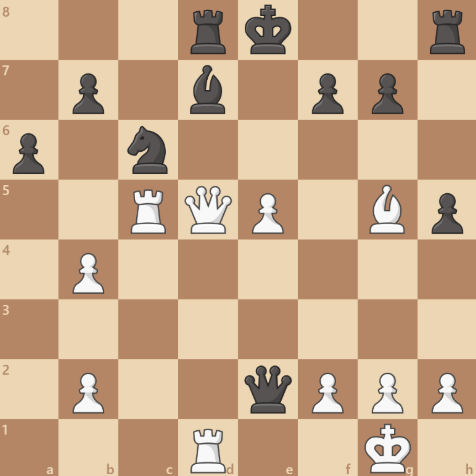
\includegraphics[width=0.35\textwidth]{../Images/Figures/Chess.png}
\end{center}
\alt<handout>{}{
\begin{itemize}
    \item<2-> En lugar de calcular cada jugada posible hasta el final, la IA usa una función para evaluar la \textbf{calidad de la posición}.
    \item<3-> Esa calidad es la probabilidad de victoria (o recompensa futura) desde esa posición.
    \item<4-> En RL, esta estimación de potencial es precisamente la \textbf{función de valor}.
\end{itemize}}
\end{frame}

% --- SLIDE: FUNCIÓN VALOR COMO TABLA ---
\begin{frame}{La Función de Valor como "Lookup Table"}
Pensemos en la función de valor como una tabla de consulta donde cada celda responde: \textit{"¿Cuánto espero ganar si empiezo ac\'a?"}

\begin{center}
    \renewcommand{\arraystretch}{1.2}
    \begin{tabular}{|l||c|c|c|}
    \hline
    \textbf{Estado ($s$)} & \textbf{Semana 0} & \textbf{Semana 1} & \textbf{Semana 2} \\ \hline \hline
    \textbf{Alcista} & $V_2(\text{Alc})$ & $V_1(\text{Alc})$ & $V_0(\text{Alc})$ \\ \hline
    \textbf{Bajista} & $V_2(\text{Baj})$ & $V_1(\text{Baj})$ & $V_0(\text{Baj})$ \\ \hline
    \textbf{Estable} & $V_2(\text{Est})$ & $V_1(\text{Est})$ & $V_0(\text{Est})$ \\ \hline
    \end{tabular}
\end{center}

\begin{itemize}
    \item<2-> Cada fila representa un estado de nuestro espacio $S$.
    \item<2-> Cada columna representa el tiempo restante o el horizonte.
\end{itemize}

\begin{block}{El Objetivo del curso}<3->
Aprenderemos algoritmos (como Programación Dinámica o RL) cuyo fin es \textbf{llenar esta tabla con los valores correctos}.
\end{block}
\end{frame}


% --- SLIDE 1: INTRODUCCIÓN A LA RECURSIÓN VISUAL ---
\begin{frame}{Recursión y el Grafo de Tiempo}
\begin{itemize}
    \item El concepto de función valor es central para la toma de decisiones.
    \item<2-> Utilizaremos la \textbf{recursión}: resolver problemas complejos dividiéndolos en sub-problemas más simples.
    \item<3-> Para visualizarlo, expandimos nuestro grafo de estados en el eje del tiempo).
\end{itemize}


\only<3>{
\begin{center}
    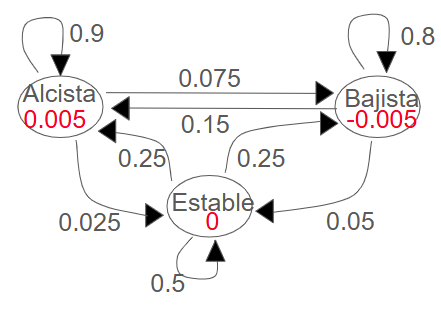
\includegraphics[width=0.55\textwidth]{../Images/Market/MarketWithReward.png}
\end{center}
}

\alt<handout>{}{
% Estilos locales para eliminar colores y ajustar el diseño
\tikzset{
    state_no_color/.style={circle, draw=black, thick, minimum size=0.8cm, font=\bfseries},
    trans/.style={->, >={Stealth[scale=1.0]}, thick, black!70, shorten >=1pt}
}

% \begin{flushleft}
\begin{tikzpicture}[node distance=2cm and 1.6cm, scale=0.8, every node/.style={scale=0.8}]

    % Ejes de tiempo (arriba) - Alineados con las coordenadas X de los nodos
    \node<4-> (t0) at (0, 3.5) {\textbf{Hoy} ($t=2$)};
    \node<6-> (t1) at (5.5, 3.5) {\textbf{Semana 1} ($t=1$)};
    \node<8-> (t2) at (11, 3.5) {\textbf{Semana 2} ($t=0$)};
    
    % Nodos de estado
    \node<4->[state_no_color] (A0) at (0, 2.5) {A};
    \node<4->[state_no_color] (B0) at (0, 0.5) {B};
    \node<4->[state_no_color] (E0) at (0,-1.5) {E};
    
    \node<6->[state_no_color] (A1) at (5.5, 2.5) {A};
    \node<6->[state_no_color] (B1) at (5.5, 0.5) {B};
    \node<6->[state_no_color] (E1) at (5.5,-1.5) {E};

    \node<8->[state_no_color] (A2) at (11, 2.5) {A};
    \node<8->[state_no_color] (B2) at (11, 0.5) {B};
    \node<8->[state_no_color] (E2) at (11,-1.5) {E};

    % Transiciones A0 -> T1
    \draw<6->[trans] (A0) to node[auto, font=\scriptsize] {0.9} (A1);
    \draw<6->[trans] (A0) to node[auto, pos=0.7, font=\scriptsize] {0.075} (B1);
    \draw<6->[trans] (A0) to node[auto, swap, pos=0.8, font=\scriptsize] {0.025} (E1);

    % Transiciones B0 y E0 -> T1 (CORREGIDO: Agregados ';' y cerrados correctamente)
    \draw<7->[trans] (B0) -- (A1);
    \draw<7->[trans] (B0) -- (B1);
    \draw<7->[trans] (B0) -- (E1);
    \draw<7->[trans] (E0) -- (A1);
    \draw<7->[trans] (E0) -- (B1);
    \draw<7->[trans] (E0) -- (E1);

    % Transiciones T1 -> T2 (CORREGIDO: Agregados ';' y simplificado el dibujo)
    \draw<8->[trans] (A1) -- (A2);
    \draw<8->[trans] (A1) -- (B2);
    \draw<8->[trans] (A1) -- (E2);
    \draw<8->[trans] (B1) -- (A2);
    \draw<8->[trans] (B1) -- (B2);
    \draw<8->[trans] (B1) -- (E2);
    \draw<8->[trans] (E1) -- (A2);
    \draw<8->[trans] (E1) -- (B2);
    \draw<8->[trans] (E1) -- (E2);

    % Etiquetas de Recompensa
    \node<5->[anchor=north, yshift=-0.1cm] (rA) at (A0.south) {\scriptsize $r(A)=0.005$};
    \node<5->[anchor=north, yshift=-0.1cm] (rB) at (B0.south) {\scriptsize $r(B)=-0.005$};
    \node<5->[anchor=north, yshift=-0.1cm] (rE) at (E0.south) {\scriptsize $r(E)=0$};

\end{tikzpicture}}
%\end{flushleft}
\end{frame}



% --- SLIDE 3: CÁLCULO PASO A PASO CON GRAFO ---
\begin{frame}{Calculando el Valor por Recursión}

\tikzset{
    state_bw/.style={circle, draw=black, thick, minimum size=0.9cm, font=\bfseries},
    trans/.style={->, >={Stealth[scale=1.0]}, thick, black!70, shorten >=1pt},
    val_label/.style={font=\tiny\bfseries, text=blue!80!black, yshift=2mm}
}

\centering

% 1. ECUACIÓN SUPERIOR: EL MODELO GENERAL
\small
\begin{itemize}
    \item<1->[] \textbf{Caso Base ($t=0$):} $V_0(s) = r(s)$ 
    \item<2->[] \textbf{Paso de Inducción ($t>0$):} $V_t(s) = r(s) + \sum_{s'} P(s,s')V_{t-1}(s')$
\end{itemize}

\vspace{0.2cm}

\alt<handout>{}{
\begin{tikzpicture}[node distance=1.8cm, scale=0.85, every node/.style={scale=0.85}]
    % Nodos de tiempo
    \node (t0) at (0, 3.2) {\textbf{Hoy} ($t=2$)};
    \node (t1) at (3.5, 3.2) {\textbf{Semana 1} ($t=1$)};
    \node (t2) at (7, 3.2) {\textbf{Semana 2} ($t=0$)};
    
    % Columna t=2
    \node[state_bw] (A0) at (0, 2) {A};
    \node[state_bw] (B0) at (0, 0.5) {B};
    \node[state_bw] (E0) at (0,-1) {E};
    
    % Columna t=1
    \node[state_bw] (A1) at (3.5, 2) {A};
    \node[state_bw] (B1) at (3.5, 0.5) {B};
    \node[state_bw] (E1) at (3.5,-1) {E};

    % Columna t=0 (Caso Base)
    \node[state_bw] (A2) at (7, 2) {A};
    \node[state_bw] (B2) at (7, 0.5) {B};
    \node[state_bw] (E2) at (7,-1) {E};

    % VALORES CASO BASE
    \node<2->[val_label] at (A2.north) {$V_0(A)=0.005$};
    \node<2->[val_label] at (B2.north) {$V_0(B)=-0.005$};
    \node<2->[val_label] at (E2.north) {$V_0(E)=0$};

    % INDICACIÓN DE REPETICIÓN - Agregado punto y coma final si faltaba en algún bloque
    \draw[trans, thin] (A1) -- (A2);
    \draw[trans, thin] (A1) -- (B2);
    \draw[trans, thin] (A1) -- (E2); 
    \draw[trans, thin] (B1) -- (A2);
    \draw[trans, thin] (B1) -- (B2);
    \draw[trans, thin] (B1) -- (E2); 
    \draw[trans, thin] (E1) -- (A2);
    \draw[trans, thin] (E1) -- (B2);
    \draw[trans, thin] (E1) -- (E2); 
    \draw[trans, thin] (A0) -- (A1);
    \draw[trans, thin] (A0) -- (B1);
    \draw[trans, thin] (A0) -- (E1); 
    \draw[trans, thin] (B0) -- (A1);
    \draw[trans, thin] (B0) -- (B1);
    \draw[trans, thin] (B0) -- (E1); 
    \draw[trans, thin] (E0) -- (A1);
    \draw[trans, thin] (E0) -- (B1);
    \draw[trans, thin] (E0) -- (E1); 

    % CÁLCULO DE V1(A)
    \draw<3-4>[trans, blue, thin] (A1) -- (A2) node[midway, above, font=\tiny] {0.9};
    \draw<3-4>[trans, blue!50, thin] (A1) -- (B2) node[pos=0.7, above, font=\tiny] {0.075};
    \draw<3-4>[trans, blue!50, thin] (A1) -- (E2) node[pos=0.8, swap, above, font=\tiny] {0.025};
\draw[trans, thin] (A1) -- (B2); 
    \draw<5-6>[trans, blue!50, thin] (B1) -- (A2) node[midway, above, font=\tiny] {};
    \draw<5-6>[trans, blue!50, thin] (B1) -- (B2) node[midway, above, font=\tiny] {};
    \draw<5-6>[trans, blue!50, thin] (B1) -- (E2) node[midway, above, font=\tiny] {}; 
    \draw<5-6>[trans, blue!50, thin] (E1) -- (A2) node[midway, above, font=\tiny] {};
    \draw<5-6>[trans, blue!50, thin] (E1) -- (B2) node[midway, above, font=\tiny] {};
    \draw<5-6>[trans, blue!50, thin] (E1) -- (E2) node[midway, above, font=\tiny] {}; 
    \draw<7-8>[trans, blue!50, thin] (A0) -- (A1) node[midway, above, font=\tiny] {};
    \draw<7-8>[trans, blue!50, thin] (A0) -- (B1) node[midway, above, font=\tiny] {};
    \draw<7-8>[trans, blue!50, thin] (A0) -- (E1) node[midway, above, font=\tiny] {}; 
    \draw<7-8>[trans, blue!50, thin] (B0) -- (A1) node[midway, above, font=\tiny] {};
    \draw<7-8>[trans, blue!50, thin] (B0) -- (B1) node[midway, above, font=\tiny] {};
    \draw<7-8>[trans, blue!50, thin] (B0) -- (E1) node[midway, above, font=\tiny] {}; 
    \draw<7-8>[trans, blue!50, thin] (E0) -- (A1) node[midway, above, font=\tiny] {};
    \draw<7-8>[trans, blue!50, thin] (E0) -- (B1) node[midway, above, font=\tiny] {};
    \draw<7-8>[trans, blue!50, thin] (E0) -- (E1) node[midway, above, font=\tiny] {}; 
    
    % VALOR CALCULADO V1(A) - CORREGIDO \node5-> a \node<5->
    \node<4->[val_label] at (A1.north) {$V_1(A)=0.009125$};
    \node<6->[val_label] at (B1.north) {$V_1(B)=-0.00825$};
    \node<6->[val_label] at (E1.north) {$V_1(E)=0$};
    
    \node<8->[val_label] at (A0.north) {$V_2(A)=0.01259$};
    \node<8->[val_label] at (B0.north) {$V_2(B)=-0.01023$};
    \node<8->[val_label] at (E0.north) {$V_2(E)=0.00219$};

\end{tikzpicture}

\vspace{0.3cm}

% 2. ECUACIÓN INFERIOR: CÁLCULO NUMÉRICO
\begin{onlyenv}<2-3>
    \begin{block}{Cálculo numérico para $V_1(A)$}
        \centering
        \small
        $V_1(A) = 0.005 + [0.9(0.005) + 0.075(-0.005) + 0.025(0)] = \mathbf{0.009125}$
    \end{block}
\end{onlyenv}}

\end{frame}

% --- SLIDE 2: INDUCCIÓN HACIA ATRÁS (TEORÍA Y TABLA BASE) ---
\begin{frame}{Funci\'on Valor Para Reg\'imenes de Mercado}

\begin{center}
\footnotesize % Ajuste de tamaño para que quepa en la slide
\renewcommand{\arraystretch}{1.3} 
\begin{tabular}{|l||c|c|c|}
\hline
\diagbox{\textbf{Estado}}{\textbf{Tiempo}} & \textbf{Hoy ($t=2$)} & \textbf{Semana 1 ($t=1$)} & \textbf{Fin ($t=0$)} \\ \hline \hline
\textbf{Alcista} & 0.01259 & 0.009125 & 0.005 \\ \hline
\textbf{Bajista} & -0.01023 & -0.00825 & -0.005 \\ \hline
\textbf{Estable} & 0.00219 & 0 & 0 \\ \hline
\end{tabular}
\end{center}
\end{frame}

% --- SLIDE 4: GENERALIZACIÓN Y MATRICES ---
\begin{frame}{Generalización Matricial del MRP}
Resolvemos el sistema completo de forma eficiente usando álgebra lineal.

\begin{alertblock}{Algoritmo de Horizonte Finito (MRP)}
Sea $\mathbf{r}$ el vector de recompensas y $P$ la matriz de transición:
\[ \mathbf{V_0} = \mathbf{r} \]
\[ \mathbf{V_t} = \mathbf{r} + P \mathbf{V_{t-1}} \quad \text{para } t=1, \dots, T \]
\end{alertblock}

\vspace{0.4cm}
\begin{itemize}
    \item Esta forma recursiva es la base de la \textbf{Programación Dinámica}.
    \item Implementación directa en Python.
    \item Nos permite llenar la tabla de valores completa para cualquier horizonte $T$.
\end{itemize}
\end{frame}


% --- SLIDE: GENERALIZACIÓN MRP ---
\begin{frame}{Resumiendo: El MRP}
Un \textbf{Proceso Markoviano con Recompensa} se define por la tupla $(S, P, r)$.

\begin{itemize}
    \item La métrica más común es la \textbf{recompensa total esperada} para un horizonte $T$:
    \[ V_T(s) = E \left[ \sum_{\tau=0}^T r(s_\tau) \mid s_0 = s \right] \]
    \item $V_t(s)$ se denomina la \textbf{funci\'on de valor}.
\end{itemize}

\visible<2->{
    \begin{block}{Algoritmo en Forma Matricial}
    Para implementar en Python, usamos vectores:
    \[ \mathbf{V_0} = \mathbf{r} \]
    \[ \mathbf{V_t} = \mathbf{r} + P \mathbf{V_{t-1}} \]
    Donde $\mathbf{V_t}, \mathbf{r} \in \mathbb{R}^{|S|}$ y $P \in \mathbb{R}^{|S| \times |S|}$.
    \end{block}
}
\end{frame}

\begin{frame}{Observaciones}
\begin{itemize}
\item Asumimos que $r$ y $P$ no dependen de $t$, entonces el proceso markoviano es homogéneo en el tiempo. Pero se puede extender el resultado al caso en que dependen de $t$: 
$$
\begin{array}{ccl}
V_0 &=& r_0 \\
V_t & = & r_t+ P_t V_{t-1},~t = 1,...,T
\end{array}
$$
\item<2-> También asumimos que la recompensa es determinística, pero podemos incorporar casos en que es aleatoria:                $$
\bar{r}(x) = {\rm E}_w\left[r(x,w)\right]
$$                          
\item<3-> Si la recompensa depende del próximo estado además del actual, también se puede incorporar utilizando: 
$$
\bar{r}(x) = {\rm E}\left[r(x,x_{t+1})| x_t = x\right] = \sum_y P(x,y)r(x,y)
$$ 
\end{itemize}
\end{frame}

% --- SECCIÓN: GESTIÓN DE INVENTARIO ---


% --- SLIDE: CONCLUSIONES Y PRÓXIMOS PASOS ---
\begin{frame}{Pr\'oximos Pasos}

\begin{itemize}
\item En la aplicaci\'on a gesti\'on de stock, ¿es nuestra estrategia $(s, S)$ la mejor posible? ¿Por qu\'e fijar el punto de reposici\'on en $n$ y no en $n-1$? ¿Por qu\'e el tope en $N$ y no el doble? ¿Es posible que otra estructura de pol\'itica obtenga mejores resultados?

\item<2->\textbf{Próxima Clase: Del MRP al MDP}
\begin{itemize}
    \item<3-> \textbf{Control Activo:} El gerente ya no sigue una regla; elige la mejor acción seg\'un el estado del mundo, adapt\'andose a m\'ultiples situaciones.
\end{itemize}
%    \item<4-> \textbf{Horizontes:} ¿Optimizar para el trimestre (finito) o para la eternidad (infinito)?
%    \item<5-> \textbf{El Tiempo es Dinero:} Introducción al \textbf{Factor de Descuento ($\alpha$)}.
%\end{itemize}
\end{itemize}
\end{frame}

%% --- SLIDE: EL FRAMEWORK DE MARKOV ---
\begin{frame}{MRPs y MDPs: Un Marco Poderoso}
Estamos ante una herramienta flexible para modelar casi cualquier escenario de **toma de decisiones secuenciales bajo incertidumbre**.

\textbf{Repaso de Componentes Clave:}
\begin{itemize}
    \item \textbf{Estado ($S$):} La informaci\'on necesaria para decidir (Propiedad de Markov).
    \item \textbf{Din\'amica ($P$):} Probabilidades de transici\'on.
   \item \textbf{Recompensa ($R$):} El feedback inmediato del entorno.
\end{itemize}

\begin{block}{La Funci\'on de Valor ($V$)}
    Es el n\'ucleo del marco: no solo mira el beneficio de hoy, sino el \textbf{acumulado esperado a futuro}. Es el puente entre la acci\'on actual y sus consecuencias a largo plazo.
\end{block}

\textit{Aplicaciones:} Log\'istica, finanzas, rob\'otica, gesti\'on de redes y m\'as.
\end{frame}
%
%% --- SLIDE: RETOS DE APLICACIÓN ---
%\begin{frame}{Retos de Implementaci\'on: De la Teor\'ia a la Pr\'actica}
%Aplicar esta metodolog\'ia en el mundo real presenta desaf\'ios formidables:
%
%\begin{itemize}
%    \item \textbf{Modelado y Abstracci\'on:} 
%    \begin{itemize}
%        \item Definir una $R$ que capture los objetivos reales sin efectos secundarios.
%        \item Estimar matrices $P$ cuando los datos son escasos o ruidosos.
%    \end{itemize}
%    
%    \item \textbf{La Elecci\'on del Estado ($S$):}
%    \begin{itemize}
%        \item El arte de incluir lo esencial y omitir lo irrelevante.
%        \item ¿C\'omo recuperar la propiedad de Markov sin inflar el modelo?
%    \end{itemize}
%
%    \item \textbf{Costo Computacional:}
%    \begin{itemize}
%        \item \textbf{Maldici\'on de la dimensionalidad:} El crecimiento exponencial del espacio de estados limita la resoluci\'on exacta.
%    \end{itemize}
%\end{itemize}
%
%\begin{exampleblock}{Reflexi\'on Final}
%    Modelar es elegir qu\'e simplificar. Un buen modelo no es el m\'as complejo, sino el que permite tomar mejores decisiones con los recursos disponibles.
%\end{exampleblock}
%\end{frame}
\end{document}

% --- SLIDE: DESAFÍOS GENERALES EN EL MODELADO DE PROCESOS ---
\begin{frame}{Retos Globales en el Modelado}
Extraigamos lecciones universales de nuestro caso de inventario:

\begin{itemize}
    \item \textbf{Fidelidad vs. Simplicidad:}
    \begin{itemize}
        \item ¿Cuándo deja de ser útil un modelo por ser demasiado simple?
        \item El riesgo de romper la \textbf{Propiedad de Markov}.
    \end{itemize}

    \item \textbf{La Maldici\'on de la Dimensionalidad:}
    \begin{itemize}
        \item El crecimiento exponencial de la matriz $P$ ante nuevas variables.
        \item ¿Resoluci\'on exacta o aproximaci\'on num\'erica?
    \end{itemize}

    \item \textbf{Incertidumbre y Datos:}
    \begin{itemize}
        \item ¿Conocemos $P$ o debemos estimarla?
        \item \textbf{Robustez:} Sensibilidad de la soluci\'on ante cambios en el entorno.
    \end{itemize}
\end{itemize}

\begin{block}{Reflexi\'on}
    El éxito de un modelo no depende de cuánto incluye, sino de qué decide ignorar.
\end{block}
\end{frame}

% --- SLIDE: CONCLUSIONES Y PRÓXIMOS PASOS ---
\begin{frame}{Conclusiones y Pr\'oximos Pasos}
\textbf{Hoy consolidamos el MRP:}
\begin{itemize}
    \item Estructura de estados, transiciones y valor.
    \item Evaluaci\'on de una pol\'itica fija $(n, N)$.
\end{itemize}

\vspace{0.4cm}
\begin{alertblock}{\textquestiondown Es nuestra pol\'itica la mejor posible?}<2->
    ¿Por qué usar esos umbrales y no otros?
\end{alertblock}

\vspace{0.4cm}
\textbf{Pr\'oxima Clase: Del MRP al MDP}<3->
\begin{itemize}
    \item \textbf{Control Activo:} El paso de seguir reglas a elegir acciones.
    \item \textbf{Horizontes:} Decisiones a corto plazo vs. operaci\'on perpetua.
    \item \textbf{Valor del Tiempo:} Introducci\'on al \textbf{Factor de Descuento ($\gamma$)}.
\end{itemize}
\end{frame}

% --- SLIDE: DISCUSIÓN FINAL - HACIA EL MDP ---
\begin{frame}{De la Evaluación al Control (MDP)}
Hasta ahora, hemos \textbf{evaluado} una política fija. Esto es un MRP.

\begin{center}
    \textbf{Pregunta crítica:} \\ ¿Es posible que reponer siempre al nivel $N$ no sea lo más rentable?
\end{center}

\vspace{0.3cm}
\textbf{Hacia el MDP (Markov Decision Process):}
\begin{itemize}
    \item El gerente ahora elige una \textbf{acción} $a_t$ (cuánto pedir).
    \item La transición y la recompensa dependen de esa acción: $P(s' | s, a)$ y $r(s, a)$.
\end{itemize}

\begin{alertblock}{Conclusión}
El MRP nos permite proyectar el valor futuro de una estrategia. El MDP nos permitirá encontrar la mejor estrategia posible.
\end{alertblock}
\end{frame}
% --- SLIDE 6: EL GRAN DILEMA ---
\begin{frame}{Exploración vs. Explotación}
¿Cómo decide un manager cuando no conoce todas las reglas?
\begin{itemize}
    \item \textbf{Explotación:} Maximizar ingresos usando la estrategia que ya sabemos que funciona.
    \item \textbf{Exploración:} Probar una nueva estrategia para \textit{aprender} si el mercado ha cambiado o si hay algo mejor.
\end{itemize}
\vspace{0.3cm}
\begin{block}{Ejemplo: Campaña de Marketing}
¿Invierto todo el presupuesto en Google Ads (Explotación) o desvío un 10\% para probar un nuevo canal en TikTok (Exploración)?
\end{block}
\end{frame}



% --- SLIDE 8: CASO MARKET SHARE (Ghana Telecom) ---
\begin{frame}{Caso de Estudio: Ghana Telecom}
Analicemos la competencia entre dos operadores: \textbf{M} y \textbf{V}.
\begin{itemize}
    \item \textbf{Lealtad M:} El 71.6% de sus clientes se quedan. El 28.4% se muda a V.
    \item \textbf{Lealtad V:} El 38.7% de sus clientes se quedan. El 61.3% se muda a M.
\end{itemize}
\vspace{0.3cm}
\textbf{Pregunta Estratégica:} Si hoy M tiene el 33% del mercado, ¿qué pasará en el largo plazo?
\end{frame}

% --- SLIDE 9: LA MATRIZ DE TRANSICIÓN ---
\begin{frame}{La Matriz de Transición ($P$)}
\[
P = 
\begin{pmatrix}
0.716 & 0.284 \\
0.613 & 0.387
\end{pmatrix}
\]
\begin{itemize}
    \item Fila 1: Probabilidades de salida de clientes de M.
    \item Fila 2: Probabilidades de salida de clientes de V.
    \item \textbf{Cálculo:} $x_{t+1} = x_t \cdot P$
\end{itemize}
\end{frame}

% --- SLIDE 10: BLOQUE 2: RECOMPENSAS ---
\begin{frame}{Definiendo el Éxito: La Recompensa ($r$)}
Un proceso de decisión necesita una señal de éxito.
\begin{itemize}
    \item No siempre es "Ventas".
    \item \textbf{¿Por qué?} Si premias ventas, el manager regalará el producto para ganar cuota.
\end{itemize}
\vspace{0.3cm}
\begin{exampleblock}{Propuesta de Recompensa}
$r(i) = \text{beneficio esperado en el estado } i$
\end{exampleblock}
\end{frame}

% --- SLIDE 11: RECOMPENSA EN INVENTARIO ---
\begin{frame}{Ejemplo de recompensa}
Una posible definición para gestión de stock:
\[ r(i) = p \cdot \mathbb{E}[\min(i, D_t)] - c \cdot i \]
\begin{itemize}
\item $p$: precio de venta por unidad.
\item $c$: costo de mantenimiento por unidad.
\item $D_t$: Demanda incierta.
\end{itemize}
\vspace{0.3cm}
\textbf{Reflexión:} ¿Por qué usamos el valor esperado? Porque el manager decide antes de conocer la demanda real.
\end{frame}

% --- SLIDE 12: EL HORIZONTE ($T$) ---
\begin{frame}{Horizonte de Decisión}
\textbf{Horizonte finito:} $t = 0, 1, \dots, T$
\begin{itemize}
\item Hay una fecha de cierre clara.
\item \textbf{Ejemplo:} Venta de ropa de temporada. Una vez que llega el invierno, la ropa de verano vale \$0.
\end{itemize}
\vspace{0.3cm}
\textbf{Horizonte infinito:} $t = 0, 1, \dots, \infty$
\begin{itemize}
\item El negocio es una operación continua (ej: mantenimiento de flota).
\end{itemize}
\end{frame}

% --- SLIDE 13: RECESO ---
\begin{frame}{Receso}
\begin{center}
    \Huge \textbf{15 MINUTOS} \\
    \vspace{0.5cm}
    \large Bloque 3: Laboratorio de Simulación.
\end{center}
\end{frame}

% --- SLIDE 14-30: BLOQUE 3: LABORATORIO (Expanded) ---
\begin{frame}[fragile]{Laboratorio: Market Share en Python}
Implementaremos el modelo de Ghana Telecom para ver la convergencia.
\begin{verbatim}
import numpy as np
import matplotlib.pyplot as plt

# Definir la matriz P
P = np.array([[0.716, 0.284], 
              [0.613, 0.387]])

# Estado inicial (M=33%, V=67%)
x = np.array([0.33, 0.67])
history = [x]
\end{verbatim}
\end{frame}

\begin{frame}[fragile]{Simulando la Trayectoria}
\begin{verbatim}
for t in range(20):
    x = np.dot(x, P)
    history.append(x)

history = np.array(history)
plt.plot(history[:, 0], label='Market Share M')
plt.plot(history[:, 1], label='Market Share V')
plt.legend()
plt.show()
\end{verbatim}
\end{frame}

\begin{frame}{Interpretación de Resultados}
\begin{itemize}
    \item ¿En qué mes se estabiliza el mercado?
    \item \textbf{Discusión:} Si eres el manager de V y quieres evitar que M domine el 68\% del mercado, ¿qué acción tomarías?
    \item Acciones posibles en el MDP:
    \begin{enumerate}
        \item Subir lealtad de V (cambiar fila 2).
        \item Robar lealtad de M (cambiar fila 1).
    \end{enumerate}
\end{itemize}
\end{frame}

\begin{frame}{El Concepto de Estado Estacionario ($\pi$)}
¿Cómo encontramos el "final del camino" sin simular 100 pasos?
\begin{itemize}
    \item Buscamos un vector $\pi$ tal que: $\pi = \pi P$
    \item En este curso aprenderemos a resolver esto para sistemas de miles de estados.
    \item Para el CEO, $\pi$ es el valor estratégico de su modelo de negocio actual.
\end{itemize}
\end{frame}

\begin{frame}{Resumen de la Clase 1}
\begin{enumerate}
    \item Los problemas de gestión son \textbf{secuenciales}.
    \item El \textbf{Estado} debe ser Markoviano.
    \item La \textbf{Recompensa} debe estar alineada con el margen, no solo con el volumen.
\end{enumerate}
\vspace{0.3cm}
\begin{alertblock}{Próxima Clase}
¿Cómo decidimos el precio óptimo? Introducción a la Ecuación de Bellman y Dynamic Programming.
\end{alertblock}
\end{frame}

\end{document}
